%!TEX root = ../BGP_for_networks_who_peer.tex
\chapter{eBGP - Connecting to the outside world}
\label{ch:eBGP}
\section{What is eBGP?}
We call a BGP session an eBGP (external BGP) session if it connects to a different Autonomous System.

\subsection{Differences between iBGP and eBGP}
There are a couple of differences between the two flavors of BGP.

One difference is that, while in iBGP it does not matter how many ``hops'' (in terms of the IP protocol) a neighbor is away, in eBGP the neighbor usually is directly connected.  You can change this behavior if you configure the neighbor as being a ``multi-hop'' neighbor (\texttt{neighbor x.x.x.x ebgp-multihop}).

\fcolorbox{black}{lgray}{
\begin{minipage}{\linewidth}
   How does it work that eBGP packets only travel to the next adjacent node?
   The answer lies with the IP \emph{TTL (Time to Live)} counter: The sender sets the counter to one, so packets get discarded if the eBGP neighbor is more then one hop away. See chapter~\ref{ch:security} to learn about a more secure approach to this.
\end{minipage}
}

Also the next-hop of IP addresses received via eBGP is set to the address the sender of the prefixes (your eBGP neighbor) specified. If you forward this prefix then via iBGP, this next hop is either unchanged or set to the IP of your router (\texttt{neighbor x.x.x.x next-hop-self}).

The router receiving a prefix via eBGP also checks if the next-hop IP address is accessible via the interface the prefix is received. If it is not, the eBGP announcement is discarded.

Your router also checks the AS-Path of all received prefixes. If your own AS number is in that path, the prefix is also discarded (this can be switched off by a config command which is \emph{not recommended}).

Other measures to ignore unwanted prefixes etc. have to be configured manually using filter lists or route-maps. More about this you can read in chapter~\ref{ch:security}.


\subsection{Best practices}
It is best practice to not let prefixes in from outside without some filtering. Most of this filtering will be covered in chapter~\ref{ch:security} when we talk about BGP security. At this time we will define empty filters for sending and receiving prefixes (named ``-out'' for sending ``-in'' for receiving). We will extend these filters later.

If your router supports it, it's again best practice to define a peer-group and have all common configuration in the peer-group (you need two peer-groups again, one for IPv4 and one for IPv6).

It is strongly recommended that you setup a filter to \emph{not announce any} prefixes initially when setting up a completely new eBGP peer group. We will do so by configuring our ``-out'' route-map to deny everything.

Depending on your routers BGP implementation, configuration commands become active the moment you hit the ``enter'' key. So if you configure an eBGP neighbor \emph{without} any filtering and the neighbor already has configure its side, you start flooding your complete BGP table immediately. \rfc{8212} addresses this problem by requesting that eBGP sessions without any \emph{configured} filtering get an automatic \emph{deny-all} filter by default. Some vendors have already implemented this, some made it optional.

Some routers allow  received information (before filter processing) to be stored in a separate table (at the cost of increased memory usage). To debug your filters, this is very useful, so I suggest you turn it on (see examples below).

\subsection{Sources and destinations of prefixes}
\begin{figure}
  \centering
  \includegraphics[width=\linewidth,page=17]{img/Drawings.pdf}
  \caption{eBGP Roles}
  \label{fig:bgproles}
\end{figure}

If you look at possible BGP neighbors, you come up with some categories you receive prefixes from and announce prefixes to. \rfc{9234} defines to following BGP neighbor roles and relationships:
\begin{description}
  \item[Provider, Customer:] A provider announces all known prefixes to a customer, a customer announces only its own and its customers prefixes to a provider.
  \item[Peer, Peer:] They announce their own and their customers prefixes to each other.
  \item[Route Server, Route Server Client:] Similar to peers, a route server announces all prefixes to a route server client, which announces their own and their customers prefixes to a route server.     
\end{description}
See picture~\ref{fig:bgproles} for a graphical expression of roles and relationships.
These relationships must be expressed in filter configurations. You can do that manually (better: automated) with allow-lists or you can implement sophisticated mechanisms. Choose what ever fits best to your network size. Chapter~\ref{ch:security} and chapter~\ref{ch:BGP Communities} will give you some ideas.

\subsection{Cisco example}
In this simple example we \emph{deny} any outgoing prefixes.
\begin{verbatim}
  route-map upstream-out deny 10
  !
  route-map upstream-in permit 10
  !
  route-map upstream6-out deny 10
  !
  route-map upstream6-in permit 10
  !
  router bgp 64500
    neigbor upstream peer-group
    neigbor upstream6 peer-group
    neighbor 192.168.3.2 remote-as 65550
    neighbor 192.168.3.2 peer-group upstream
    neighbor 2001:db8:300::2 remote-as 65550
    neighbor 2001:db8:300::2 peer-group upstream6
    !
    address-family ipv4
      neigbor upstream route-map upstream-in in
      neigbor upstream route-map upstream-out out
      neigbor upstream soft-reconfiguration inbound
      neigbor upstream6 route-map upstream6-in in
      neigbor upstream6 route-map upstream6-out out
      neigbor upstream6 soft-reconfiguration inbound
      neighbor 192.168.3.2 activate
      no neighbor 2001:db8:300::2 activate
    !
    address-family ipv6
      neigbor upstream route-map upstream-in in
      neigbor upstream route-map upstream-out out
      neigbor upstream soft-reconfiguration inbound
      neigbor upstream6 route-map upstream6-in in
      neigbor upstream6 route-map upstream6-out out
      neigbor upstream6 soft-reconfiguration inbound
      no neighbor 192.168.3.2 activate
      neighbor 2001:db8:300::2 activate
\end{verbatim}
The \emph{soft-reconfiguration inbound} ensures that you can check what your router receives before it is processed by the incoming route-map.

Take note of how the address-family parts and entry act together. ``address-family'' relates to the \emph{announced} prefixes; the IP address of the neighbor defines the protocol of the BGP session. With the ``activate'' clauses we switch off IPv4 prefix announcement on the IPv6 sessions and switch on IPv6 announcement. On the IPv4 sessions, we do it the other way around. What increases the confusion is that some of these statements are considered to be default at Cisco and therefore are omitted in the config.

Do we need different route-maps for IPv4 and IPv6? That's dependent on their complexity. \emph{If} you want to do any IP related filtering (ip address lists, prefix lists) having two (or four) route-maps is recommended.

\subsection{Mikrotik example}
\begin{verbatim}
  /routing bgp instance
  set default as=64500 router-id=192.168.1.1

  /routing bgp peer
  add name=upstream-AS65550 in-filter=upstream-in \
    out-filter=upstream-out \
    remote-address=192.168.3.2 remote-as=65550
  add name=upstream6-AS65550 in-filter=upstream6-in \
      out-filter=upstream6-out \
      remote-address=2001:db8:300::2 remote-as=65550 \
      address-families=ipv6

  /routing filter
  add chain=upstream-in action=accept
  add chain=upstream-out action=discard
  add chain=upstream6-in action=accept
  add chain=upstream6-out action=discard
\end{verbatim}
Mikrotik does not support peer-groups or similar, so everything needs to be configured on every peer. Here the ``address-families'' parameters determines what kind of prefixes are announced and accepted. Again, the default ``IPv4 only'' can be omitted - making the configuration rather more then less confusing.

We also do not announce any prefixes here (by using the \emph{action=discard} statement in our filters).

\subsection{FRRouting example}
In FRRouting we can put the \emph{activate} clauses into the peer group, also we enable \rfc{8212} automatic filtering:
\begin{verbatim}
route-map upstream-out deny 10
!
route-map upstream-in permit 10
!
route-map upstream6-out deny 10
!
route-map upstream6-in permit 10
!
router bgp 64500
  bgp ebgp-requires-policy
  neigbor upstream peer-group
  neigbor upstream6 peer-group
  neighbor 192.168.3.2 remote-as 65550
  neighbor 192.168.3.2 peer-group upstream
  neighbor 2001:db8:300::2 remote-as 65550
  neighbor 2001:db8:300::2 peer-group upstream6
  !
  address-family ipv4
    neigbor upstream route-map upstream-in in
    neigbor upstream route-map upstream-out out
    neigbor upstream soft-reconfiguration inbound
    neighbor upstream activate
    neigbor upstream6 route-map upstream6-in in
    neigbor upstream6 route-map upstream6-out out
    neigbor upstream6 soft-reconfiguration inbound
    no neighbor upstream6 activate
  exit-address-family
  !
  address-family ipv6
    neigbor upstream route-map upstream-in in
    neigbor upstream route-map upstream-out out
    neigbor upstream soft-reconfiguration inbound
    neigbor upstream6 route-map upstream6-in in
    neigbor upstream6 route-map upstream6-out out
    neigbor upstream6 soft-reconfiguration inbound
    no neighbor upstream activate
    neighbor upstream6 activate
  exit-address-family
\end{verbatim}
% \subsection{Juniper example}
